\documentclass[12pt]{article}
\usepackage{graphicx}
\def\baselinestretch{1.5}
\setlength{\topmargin}{0pt}
\setlength{\textheight}{570pt}
\setlength{\oddsidemargin}{0pt}
\setlength{\evensidemargin}{60pt}
\setlength{\textwidth}{427pt}
%\setlength{\footheight}{0pt}
\setlength{\footskip}{30pt}
\parindent 15pt
\hyphenpenalty=10000
\tolerance=10000
\pagestyle{plain}

\begin{document}
\newcommand{\prob}{{\rm\;Prob\;}}
\begin{bf}
\vspace{1in}

\centerline{A Hidden Markov Model Approach to Variation Among Sites}
\centerline{in Rate of Evolution}
\vspace{0.5in}

\end{bf}

\centerline{Joseph Felsenstein\(^{*,}\)\footnotemark ~and Gary A. Churchill\(^{\dag,}\)\footnotemark}
\bigskip

\noindent
\(^*\)Department of Genetics, University of Washington, Seattle, Washington 98195 and\\
\(^{\dag}\)Department of Plant Breeding and Biometry, Cornell University, Ithaca, New York 14853

\vspace{0.5in}


\footnotemark[1]Internet address: joe@genetics.washington.edu

\footnotemark[2]Internet address: gary@amanita.biom.cornell.edu


\vspace{0.4in}

\centerline{Running Head:  Likelihood and evolutionary rates}
\bigskip



{\it Key words:}  likelihood, phylogeny, statistical inference, hidden Markov
model, rate of evolution, molecular sequences
\bigskip

\begin{flushleft}
Corresponding Author:\\
\medskip

Joe Felsenstein\\
Department of Genetics SK-50\\
University of Washington\\
Seattle, WA 98195, USA\\
\medskip
Phone: (206) 543-0150\\
Fax: (206) 543-0754\\
Internet: joe@genetics.washington.edu
\end{flushleft}

\newpage

\centerline{\bf Abstract}

The method of hidden Markov models is used to allow for unequal and unknown
evolutionary rates at different sites in molecular sequences.  Rates of
evolution at different sites are assumed to be drawn from a set of possible
rates, with a finite number of possibilities.  The overall likelihood of a
phylogeny is calculated as a sum of terms, each term being the probability
of the data given a particular assignment of rates to sites, times the
prior probability of that particular combination of rates.  The probabilities
of different rate combinations are specified by a stationary Markov chain that
assigns rate categories to sites.  While there will be a very large number
of possible ways of assigning rates to sites, a simple recursive algorithm
allows the contributions to the likelihood from all possible combinations of
rates to be summed, in a time proportional to the number of different rates
at a single site.  Thus with 3 rates, the effort involved is no greater than
3 times that for a single rate.  This ``hidden Markov model" method allows for
rates to differ between sites, and for correlations between the rates of
neighboring sites.  By summing over all possibilities it does not require
us to know the rates at individual sites.  However it does not allow for
correlation of rates at non-adjacent sites, nor does it allow for a
continuous distribution of rates over sites.  It is shown how to use the
Newton-Raphson method to estimate branch lengths of a phylogeny, and to infer
from a phylogeny what assignment of rates to sites has the largest posterior
probability.  An example is given using $\beta$-hemoglobin DNA sequences
in 8 mammal species; the regions of high and low evolutionary rates are
inferred and also the average length of patches of similar rates.

\newpage

\section*{Introduction}

It has long been recognized that the assumption of equal rate of
evolution implicit in many methods of analyzing phylogenies from
molecular data is unrealistic.  Maximum likelihood methods of
inferring phylogenies from molecular sequences have always made this
assumption (Neyman, 1971; Felsenstein, 1981).   It is also implicit
in almost all distance matrix methods using molecular sequences
(e.g. Jukes and Cantor, 1969; Kimura, 1980).  By assuming a given
prior distribution of rates among sites one can correct these
distance matrix methods for rate variation among sites (Olsen, 1987;
Jin and Nei, 1990).  However, such corrections do not
restrict the effect of rate variation so that the same sites are
inferred to have high rates of evolution across all members of the
set of sequences.  They also do not allow for any
correlation in rates of evolution along the molecule.

Maxmimum likelihood methods can allow for variation in rates of
evolution.  For example, the PHYLIP package distributed by one of
us (J.F.) has, in its DNAML and DNAMLK programs, versions 3.1 to 3.4, 
a ``Categories" option
that allows us to decide which rate category each site falls
into, with the relative rates of evolution in different categories
specified by us.  This assumes that we know the relative
rates of evolution in different sites, which is often not the case.
Distance matrix methods can also be modified to allow for such site-specific
rates, as is done in the program DNADIST in PHYLIP 3.5.

A halfways realistic treatment of rate variation among sites would
have the following properties:
\begin{enumerate}
\item It must allow rates to differ among sites.
\item It must not assume that we know the relative rates
of change at the individual sites, but must instead infer these
from the data.
\item It must allow there to be some correlation between the
rates of evolution at adjacent sites.
\end{enumerate}

We will describe here a method of carrying out maximum likelihood
estimation of phylogenies which satisfies these criteria.  It
will assume that there are a discrete set of possible rates (for
example, one could assume that there were four different possible
rates of evolution that stood in the ratios 0 : 1 : 2.3 : 8.9).  It will
also assume that we can assign prior probabilities to these different
rates, so that we feel able to say that the probability that a given
site is in these four categories is (say) 0.10 : 0.32 : 0.22 : 0.36.  But
we will not assume that we know which category of rate any
given site is in.  Furthermore we will allow correlation of rates among
sites which are adjacent in the molecule.

We note that Yang (1993) and Kelly and Rice (1995) have developed methods of
analyzing rate
variation in a maximum likelihood analysis of phylogeny that satisfy
conditions (1) and (2) above, and allow for a potentially infinite
number of rate categories, so that we do not need to place any
prior restriction on which rates are possible.  This great generality is
achieved at a cost: condition (3) is not met, and their calculations
become difficult beyond a small number of species.  Our approach will
be less general in the rates it allows, but more general in allowing
autocorrelation and in being useable in cases with many species.  Yang (1994)
has tested a similar discrete approximation, replacing a gamma
distribution of rates by a discrete distribution with four well-chosen
classes, and found it to perform well.

Our method uses the method of Hidden Markov Models (Baum and Petrie, 1966)
which has been widely used in signal processing in communications,
and was first applied to
molecular sequences by Churchill (1989).  Hidden Markov Models have
also recently been applied to inferences of 
sequence alignment of proteins (Haussler et. al., 1993; Baldi et. al., 1994;
Krogh et. al., 1994).  Krogh et. al. also refer to some
other recent applications of Hidden Markov Models to molecular biology.

The method we describe requires an amount of computation that is
greater than that for simple maximum likelihood inference of phylogenies
by a factor roughly equal to the number of different rate
categories.  Thus, in the four-category example mentioned above,
the amount of computation required to infer phylogenies is roughly four
times as great as with a single rate.  The method is implemented in
versions 3.5 and later of the programs DNAML and DNAMLK in the PHYLIP package,
which have been in distribution since March of 1993.

The present methods are quite similar to the auto-discrete-gamma model
of Yang (1995), which was developed independently of them.  He has used a
bivariate Gamma distribution to model
autocorrelation of rates among sites, and in order to effectively approximate
this model has derived from it an autocorrelated Hidden Markov Model of
rate variation.  His model differs in detail from the present model but is
similar in logical structure, and may give similar estimates of the phylogeny.

In this paper we outline the theory and computational methods for
computing likelihood for a phylogeny with evolutionary rates that follow
a Hidden Markov Model.  We then explain the model of base substitution
that is used in our implementation of this method, and the method of
searching for the tree of highest likelihood, using a Newton-Raphson
method that is specific to that base substitution model.  We also
also give a data example using mammalian hemoglobin sequences.

\section*{The model}

The variation in evolutionary rates in our model is laid down by a Markov
process that operates along the molecule, and assigns rates to sites.  The
rates are chosen from a finite pool of available rates, and the
Markov process is assumed to be stationary and irreducible, so that we can talk of the
equilibrium probabilities $f_i$ of the rates.  The transition probabilities
$P_{ij}$ of this Markov process are assumed to be known.  This Markov process
is hidden from our view, as we cannot directly observe 
which sites evolve at which rates.

Once the sites have their rates assigned, each site will be assumed to
evolve independently along the true phylogeny with that rate.  Figure 1
depicts the model.  Thus all
correlation between sites will be assumed to be the consequence of the
clustering (if any) of high and low rates at adjacent sites.  A more complex
model would be needed to deal with
causes of correlation such as compensating substitutions in RNAs,
both because the members of the pair of sites undergoing compensating
substitutions may be widely separated along the molecule, and because the
actual evolutionary events at the sites show a dependence that goes beyond
their assignment to the same rate category.

The likelihood of a given phylogeny $T$ is the sum, over all assignments of
rate categories, of the probability of the data $D$ given that combination of
rates, multiplied by the prior probability of that combination of rates.  If
$c_i$ denotes the category that a given rate combination assigns to site $i$,
so that the rate assigned to site $i$ is $r_{c_i}$, then if there are $n$
sites we may write the
likelihood of a given phylogeny as
\begin{equation} %1
L = \prob (D|T) = \sum_{c_1} \sum_{c_2} ... \sum_{c_n} \prob(c_1, c_2, ... c_n) \prob(D|T, r_{c_1}, r_{c_2}, ..., r_{c_n}).
\end{equation}
The assumption that each site evolves independently once
the rate categories $c_i$ are determined allows us to express the last
probability as a product of terms, so that if $D_i$ are the data at site $i$,
\begin{equation} %2
L = \sum_{c_1} \sum_{c_2} ... \sum_{c_n} \prob(c_1, c_2, ..., c_n) \prod_{i=1}^n
\prob(D_i|T, r_{c_i}).
\end{equation}

\section*{Simplifying the calculation}


The hidden Markov model specifies that each combination of rate categories
$c_1, c_2, ... c_n$ is the outcome of a stationary Markov chain, and thus its
prior probability is simply the product of the prior probability of $c_1$
times a product of transition probabilities of that Markov chain:
\begin{equation} %3
\prob (c_1, c_2, ..., c_n) = f_{c_1} P_{c_1, c_2} P_{c_2, c_3} ... P_{c_{n-1},c_n}
\end{equation}
It might be thought that there would be severe problems in computing (2), as,
if there are $k$ rate categories, the number of combinations of categories will
be $k^n$.  Thus with 1000 sites and 3 rate categories there are $3^{1000} \simeq
10^{477}$ terms to sum.  In fact, the calculation can be done far more easily,
using an algorithm that is similar in structure to the algorithm that
calculates likelihood along a phylogeny.
Let us denote by $D^{(k)}$ the data set consisting of sites $k$ through $n$ only.
Then we can use (3) to write the likelihood as 
\begin{equation} %4
L = \sum_{c_1}f_{c_1}\left(\sum_{c_2} \sum_{c_3} ... \sum_{c_n} \prob(c_2, ... c_n|c_1) \prob(D|T, r_{c_1}, r_{c_2}, ..., r_{c_n})\right)
\end{equation}
and then use (2) to rewrite it as 
\begin{equation} %5
L = \sum_{c_1}f_{c_1}\left(\sum_{c_2} \sum_{c_3} ... \sum_{c_n} \prob(c_2, ... c_n|c_1) \prod_{i=1}^n\prob(D_i|T, r_{c_i})\right).
\end{equation}
The term in parentheses on the right-hand-side of (5) is the likelihood
of the tree for $D^{(1)}$, given that site 1 has rate category $c_1$.  Let
us call this conditional likelihood $L_{c_1}^{(1)}$.  We will, more generally,
define $L_{c_k}^{(k)}$ as the likelihood of $T$ for the data $D^{(k)}$ given that
site $k$ has rate category $c_k$.  Then
\begin{equation}%6
L = \sum_{c_1} f_{c_1} L_{c_1}^{(1)}.
\end{equation}

We can use equation (2) to write
\begin{equation} %7
L_{c_1}^{(1)} = \prob(D_1|T, r_{c_1})\sum_{c_2} \sum_{c_3} ... \sum_{c_n} \prob(c_2, ... c_n|c_1) \prod_{i=2}^n\prob(D_i|T, r_{c_i}).
\end{equation}
Equation (3) now allows us to write
the conditional probability of $c_2, c_3, ..., c_n$ given
$c_1$ as $P_{c_1,c_2}P_{c_2,c_3} ... P_{c_{n-1},c_n}$ which allows us to
rewrite $L_{c_1}^{(1)}$ as
\begin{equation} %8
L_{c_1}^{(1)} = \prob(D_1|T, r_{c_1})\sum_{c_2} P_{c_1,c_2} \left(\sum_{c_3} ... \sum_{c_n} \prob(c_2, ... c_n|c_1) \prod_{i=2}^n\prob(D_i|T, r_{c_i})\right).
\end{equation}
Noting that the expression in parentheses on the right-hand-side of (8) is just
$L_{c_2}^{(2)}$, we have an expression for the $L_{c_1}^{(1)}$ in terms of the $L_{c_2}^{(2)}$:
\begin{equation}%9
L_{c_1}^{(1)} = \prob(D_1|T, r_{c_1})\sum_{c_2} P_{c_1,c_2} L_{c_2}^{(2)}.
\end{equation}

This suggests that a general recursion might exist, calculating
each of the $L_{c_k}^{(k)}$ in terms of the $L_{c}^{(k+1)}$, and in fact
this is easily shown by continuing the same argument, repeatedly using (2) and
(3), that
\begin{equation}%10
L_{c_k}^{(k)} = \prob(D_k|T, r_{c_k})\sum_{c_{k+1}} P_{c_k,c_{k+1}} L_{c_{k+1}}^{(k+1)}.
\end{equation}
The exception to this equation is when $k = n$, in which case by definition
\begin{equation}%11
L_{c_n}^{(n)} = \prob(D_n|T, r_{c_n}).
\end{equation}

The pattern of computation reverses the order of the recursion in equation (10).
First, we must compute all the $\prob(D_k|T, r_{c_k})$, which are the
likelihoods at each site for each possible rate category.  The amount of
computation for this will be proportional to the product of the number of
sites and the number of rate categories.
Then we use (11) to determine the values of the $L_{c_n}^{(n)}$.  Then (10) can
be used to compute $L_{c_{n-1}}^{(n-1)}, L_{c_{n-2}}^{(n-2)}$, and so on
down to $L_{c_1}^{(1)}$.  There are $n-1$ steps in this computation, each
one in the most general case requiring an effort proportional to the square of the number of rate
categories.  Finally equation (6) is used to compute $L$.  The storage
requirements of this computation are modest: we can store all of the
values of $\prob(D_k|T, r_{c_k})$, there being $n$ times the number of
rate categories of these.  The computation can be done with less storage than
this, although in most cases that economy will be unnecessary.

The computation described here proceeds from the last site, $n$ to the first
one.  It could just as easily be done in the other direction, in which case
the formulas would be analogous, $P_{ij}$ being replaced by the reverse
transition probability $Q_{ji}$, where we have the usual formula for
computing the transition probabilities for the reversed Markov chain
\begin{equation}%12
Q_{ji} = f_i P_{ij} / f_j.
\end{equation}
If the Markov chain is reversible, then the $Q_{ij}$ and the $P_{ij}$ will
be identical.

As stated here, the computation may require effort proportional to the
square of the number of rate categories.  However, for the particular choice
of $P_{ij}$ used in our implementation of this method, described below,
the computation in equation (10) can be done in a time linear in the
number of rate categories.


\section*{The most probable combination of rates}

Our ability to calculate the likelihood of the phylogeny $T$ allows us to
search for the maximum likelihood phylogeny.  Once that is estimated, we
may want to see some indication of what the rates of evolution are at
the different sites.  The likelihood has been computed by summing contributions
from all possible combinations of rates.  One combination that may be of
particular interest is the combination that makes the largest contribution
to the likelihood.  This will depend on both the prior probability of the
combination and the likelihoods at the sites, as its contribution will be:
\begin{equation} %13
R =  \max_{c_1, c_2, ..., c_n} \prob(c_1, c_2, ... c_n) \prob(D|T, r_{c_1}, r_{c_2}, ..., r_{c_n}).
\end{equation}

There is an algorithm, closely related to the one used to sum likelihoods in
the previous section, that finds the combination of rates that achieves this
maximum.  It is a version of the algorithm of Viterbi (1967), which is well
explained by Forney (1973).  In an analogue to
the quantity $L_{c_i}^{(i)}$ of the previous section, let us define $R_{c_k}^{(k)}$
as the likelihood contribution for sites $k$ through $n$ for the combination
of rates that has site $k$ having rate category $c_k$, and sites $k+1$ through
$n$ having that combination of categories that maximizes the contribution of
sites $k$ through $n$, so that we define
\begin{equation} %14
R_{c_k}^{(k)} =  \max_{c_{k+1}, ..., c_n} \prob(c_{k+1}, ... c_n | c_k) \prob(D^{(k)}|T, r_{c_k}, r_{c_{k+1}}, ..., r_{c_n}).
\end{equation}
For $k=n$ the definition (14) specifies that
\begin{equation}%15
R_{c_n}^{(n)} = \prob(D_n|T, r_{c_n})
\end{equation}
which we have already calculated.  For all other values of $k$ we have a
relation analogous to (10), but taking maxima rather than summing the contributions:
\begin{equation}%16
R_{c_k}^{(k)} = \prob(D_k|T, c_k)\max_{c_{k+1}} \left[ P_{c_k,c_{k+1}}R_{c_{k+1}}^{(k+1)}\right].
\end{equation}
Using this successively on sites $n-1$, $n-2$, and so on down to 1, we end up
with the $R_{c_1}^{(1)}$ for all possible categories $c_1$ for site 1.  The largest
of the quantities $f_{c_1} R_{c_1}^{(1)}$ is the size of the largest contribution of a single combination of rate categories to the likelihood.

This leaves us without yet knowing the combination of categories
$c_1, c_2, ..., c_n$ that achieved this maximum.  However, as we used equation
(16) for each site we computed, for each possible rate category at that site,
the rate category $c_{k+1}$ at the next site that maximized the contribution.  Suppose
that we call this $C_{c_k}^{(k)}$, so that $C_{c_k}^{(k)}$ is the value of $c_{k+1}$
that is selected by the maximization in equation (16).  These values of
$c_{k+1}$ can be stored in the array $S$ as the computation proceeds from
site $n$ down to site 1.  At the end we know which rate category $c_1$
corresponds to the maximum contribution.  We can then use $C_{c_1}^{(1)}$
to find the value of $c_2$ that is involved in the maximum contribution, and
then $C_{c_2}^{(2)}$ specifies the category for site 3, and so on.
Backtracking in this way we quickly read off the combination of rate
categories that makes the largest contribution, and report these.

The combination of rate categories that makes the largest contribution to the
likelihood is not necessarily the only one that might be of interest.  We might
also imagine finding, for each site, the rate category at that site that
is involved in making the largest total contribution to the likelihood (so that
the sum of the contributions of all combinations of rate categories that have
category $c_k$ at site $k$ is as large as possible).  If for each combination
of rate categories we divide their contribution to the likelihood by the
overall likelihood, these quantities will sum to 1, and we can consider them
as a probability distribution.  The quantity $R$ we were computing
in equations (14)-(16)
is the size of the mode of that distribution.  The present quantity is in effect
for each site $k$ the mode of the marginal distribution
over $c_k$.  In general, the categories
that together make the largest contribution to the likelihood will usually also
be the ones that individually make the largest site-by-site marginal contribution, but
there can be cases in which the two methods will select different combinations
of rates.  We will see below that it is not hard to compute the combination of rate categories
that have the largest marginal contributions, using an algorithm similar to
those given above, but making two passes through the sites, one from $n$ down
to 1, and one back up again.

\section*{The implementation}
 
The discussion above applies to any stationary Markov process for assigning
rates to sites, and any Markov process that has such rates as a parameter and
that controls the evolution of sites at those rates on a given phylogeny.  The
hidden Markov model method for allowing for rate variation has been implemented
in version 3.5 of the programs DNAML and DNAMLK in the PHYLIP Phylogeny
Inference Package, which is distributed by one of us (J.F.) and is available
for free, including distribution over Internet by anonymous ftp from
evolution.genetics.washington.edu.  This version was first
made available in March, 1993.  While we emphasize
that the general method applies to many other models, in this section we will
give some details of the particular models used in these programs.

We are allowed to specify the number of different rate categories that
will be possible, the relative rates $r_i$ of the different categories, and
the equilibrium probabilities $f_i$ of each category.  The $r_i$ may be any
nonnegative real numbers, and the $f_i$ any set of frequencies that add to
1.  Note that we can allow for invariant sites by simply having one category
that has $r_i = 0$.  There also is an autocorrelation parameter,
which we will call $\lambda$.
Each site is assumed to have a probability $\lambda$ that the rate at that
site is the same as at the previous site.  With probability $1-\lambda$ the
rate is instead drawn at random from the equilibrium distribution of rates,
including the possibility that the same rate is drawn again by chance.

It is possible to estimate the values of the relative rates $r_i$ and probabilities $f_i$
and the autocorrelation parameter $\lambda$, using the EM algorithm
of Baum et al. (1970).
However implementation of this algorithm for the rates would significantly
increase computation required (it could more readily be used to
estimate the autocorrelation parameter alone). 
We have found in practice that it is more efficient
to examine a few sets of rates and correlation values
and choose one that yields the highest likelihood.

The transition probability, under this model, from state $i$ to state $j$
will be
\begin{equation}%17
P_{ij}  =  \lambda \delta_{ij} + (1 - \lambda) f_j
\end{equation}
where $\delta_{ij}$ is the Kronecker delta function, which is 1 when
$i = j$ and 0 otherwise.  This model will achieve the stated equilibrium
distribution $f$ of rate categories.  If $\lambda$ is near 1 there will
be a large autocorrelation of rate categories among neighboring sites; if
it is 0 there will be no autocorrelation.  The expected size of a patch of
sites would be $1/(1-\lambda)$, except that there is nothing in this model
that prevents the next rate category that is chosen from being the same as
the present one.  The overall probability that the rate does not change
from one site to the next is the weighted average of the $P_{ii}$:
\begin{equation}%18
\sum_i f_i P_{ii}  =  \lambda  + (1 - \lambda) \sum_i f_i^2.
\end{equation}
and this value can be used to compute the mean apparent patch size.
If there are two rate categories of equal frequency, this number is
$(\lambda+1)/2$.  If there are 10 categories of equal frequency, it is
$(0.9\;\lambda+0.1)$, which is much closer to the value of $\lambda$ that
would hold if adjacent patches never accidentally had the same rate.
In the DNAML and DNAMLK implementations, we are asked to specify an
``average patch length", but this is actually taken to be $1/(1-\lambda)$, and $\lambda$ is
set from its value.  In view of equation (18) this will be slightly incorrect.

\section*{The model of base change used in the programs}

The computational scheme presented above will work for any model of
base change for which we can specify evolutionary rates that may differ from
site to site.  In most models this is easily done by allowing the
branch lengths in the phylogeny to be proportional to 
the rates of evolution (and thus to differ from site to site).  In effect,
we treat a site that has twice the rate of evolution as if it evolves
along a branch that is twice as long.  Thus if we have a model of evolution
that has a transition probability that depends on both branch length $t$
and evolutionary rate $r$ so that it is $M_{ij}(t, r)$, the rates can be
accomodated by multiplying the branch length by $r$ if and only if
\begin{equation}%19
M_{ij}(t, r) = M_{ij}(rt, 1)
\end{equation}
This is true for most models of base change, as they accomodate site-specific
rates of evolution by replacing the time $t$ by the product $r_kt$ for site $k$.

The particular model that we have used in DNAML and DNAMLK version 3.5 is
one that allows for inequalities of equilibrium base composition and for
inequalities of the rate of transitions and transversions.  It is related to
the model given by Felsenstein (1981) but generalizes it to allow for
unequal rates of transitions and transversions.  Hasegawa, Kishino and Yano
(1988; also Kishino and Hasegawa, 1989) have previously described this model
in print, in the course of
describing their own model that also allows for inequalities of base
composition and transition/transversion rates.  Their model is similar
to the present one but not identical to it; in practice the similarity was such
that they were willing to
use the present model in many of their likelihood computations using programs
from the PHYLIP package.  A similar but not identical model has also been
developed by Rempe (1988).  The present model has been
used by J.F. in versions of the PHYLIP package distributed since 1984. 

The model can be described as having two kinds of event, I and II.  The
first can generate either no change or a transition, the second no change,
a transition, or a transversion.  Suppose that the rates of these two events
are called $\alpha$ and $\beta$.  Event I is the replacement of the
nucleotide at the site by one that is randomly sampled from the equilibrium
pool of purines (if the original base is a purine) or pyrimidines (if the
original base is a pyrimidine).  For example, a base which is an $A$
is replaced by another $A$ with probability $\pi_A/(\pi_A+\pi_G)$, and
with a $G$ with probability $\pi_G/(\pi_A+\pi_G)$.  A base which is a $C$
is replaced by another $C$ with probability $\pi_C/(\pi_C+\pi_T)$, and
with a $T$ with probability $\pi_T/(\pi_C+\pi_T)$.  Thus an event of type I
may either cause no change or a transition.

An event of type II replaces the base with one drawn from the pool of all
four possible nucleotides, with probabilities equal to their equilibrium
base composition.  Thus an $A$ is replaced by another $A$ with probability
$\pi_A$, by a $G$ with probability $\pi_G$, by a $C$ with probability $\pi_C$,
and by a $T$ with probability $\pi_T$.  An event of type II can case no
change, a transition, or a transversion.

The overall rate of substitution per site will be
\begin{equation}%20
\begin{array}{c}
\mu = \alpha \left(\pi_A \left(\frac{\pi_G}{\pi_A+\pi_G}\right) + \pi_G \left(\frac{\pi_A}{\pi_A+\pi_G}\right) + \pi_C \left(\frac{\pi_T}{\pi_C+\pi_T}\right)
+\pi_T \left(\frac{\pi_C}{\pi_C+\pi_T}\right)\right)\\
\\
 + \beta (\pi_A (1-\pi_A) + \pi_G (1-\pi_G) +
\pi_C (1-\pi_C) + \pi_T (1-\pi_T)).
\end{array}
\end{equation}
If $\pi_R$ and $\pi_Y$ are the equilibrium base frequencies of purines and
pyrimidines, respectively, so that
\begin{equation}%21
\pi_R = \pi_A + \pi_G
\end{equation}
and
\begin{equation}%22
\pi_Y = \pi_C + \pi_T,
\end{equation}
then we can simplify (20) to become
\begin{equation}%23
\mu = \alpha \left(2\pi_A\pi_G/\pi_R+2\pi_C\pi_T/\pi_Y\right)+\beta \left(1-\pi_A^2-\pi_G^2-\pi_C^2-\pi_T^2\right).
\end{equation}

The ratio of transitions to transversions will be
\begin{equation}%24
R = \left(\alpha \left(2\pi_A\pi_G/\pi_R+2\pi_C\pi_T/\pi_Y\right)+\beta \left(2\pi_A\pi_G+2\pi_C\pi_T\right)\right)/\left(\beta 2\pi_R\pi_Y\right).
\end{equation}

Expressing the instantaneous rates of transition $b_{ij}$ between the different nucleotides in terms
of the rates $\alpha$ and $\beta$ of type I and type II events we get for any
two bases $i$ and $j$
\begin{equation}%25
b_{ij} = -\delta_{ij} (\alpha+\beta) + \epsilon_{ij} \alpha \frac{\pi_j}{\sum_k \pi_j \epsilon_{jk}} + \beta \pi_j,
\end{equation}
where $\delta_{ij}$ is the usual Kronecker delta function, and $\epsilon_{ij}$
is a similar function which is 1 when $i$ and $j$ are either both purines
or both pyrimidines, and 0 otherwise.  Note that the term $\sum_k \pi_j \epsilon_{jk}$ simply computes either $\pi_R$ or $\pi_Y$, depending on whether $j$ is a
purine or a pyrimidine.  This parameterization of the model is
essentially the same as that given by Hasegawa, Kishino, and Yano (1988).

Solving (23) and (24) for $\alpha$ and $\beta$, we get
\begin{equation}%26
\alpha  =  \frac{2\pi_R\pi_Y R - (2\pi_A\pi_G+2\pi_C\pi_T)}{(2\pi_A\pi_G/\pi_R+2\pi_C\pi_T/\pi_Y)}\frac{\mu}{1+R}
\end{equation}
and
\begin{equation}%27
\beta  =  \frac{1}{2\pi_R\pi_Y}\frac{\mu}{1+R}.
\end{equation}
We can express the instantaneous rates (25) in terms of $\mu$ and $R$
by substituting (26) and (27) into (25).  The results are straightforward and
not particularly edifying and we will not give them here.

An advantage of the present model is that it is easy to compute transition
probabilities for any time $t$.  If there has been at least one event of type
II during this time, the probability of resulting base being $j$ is simply
$\pi_j$, regardless of how many other events of either type have also
occurred.  If there has been no event of type II but at least one event of
type I, the probability of the resulting base being $j$ is simply $\pi_j/\sum_k \pi_j \epsilon _{ik}$, regardless of how many other events of type I have
occurred.  As the probability of at least one event of type II is $1-\exp(-\beta t)$, and the probability of no event of type II but at least one of type I
is $\exp(-\beta t) (1-\exp(-\alpha t))$, the transition probabilities can be
given as
\begin{equation}%28
M_{ij}(t, 1) = e^{-(\alpha+\beta)t} \delta_{ij} + e^{-\beta t} \left(1-e^{-\alpha t}\right)\left(\frac{\pi_j}{\sum_k
\pi_j \epsilon _{ik}}\right) \epsilon_{ij} + \left(1-e^{-\beta t}\right) \pi_j,
\end{equation}
and they can be re-expressed in terms of the more meaningful parameters $\mu$
and $R$ by substituting from (22) and (23) for $\alpha$ and $\beta$.


\section*{Evaluating the likelihoods along the tree}

Given that we can evaluate the likelihood of any given tree $T$ for any
given parameter value $\lambda$, we still have to solve the problem of
maximizing the likelihood over all $T$ and all $\lambda$.  In practice the
methods used in DNAML version 3.5 and DNAMLK version 3.5 are not sophisticated.
Many of the particulars have been described earlier (Felsenstein, 1981)
although the program in current distribution differs in many ways from that
described in 1981.  For a given phylogeny in DNAML each branch length is
iterated separately
(in DNAMLK each ancestral node time is iterated separately), using
the Newton-Raphson method, repeatedly evaluating the likelihood.  This does
not require a re-evaluation of likelihoods throughout the tree each time,
because the ``pruning" algorithm can be used.

This algorithm, a relative of the ``peeling" algorithm in statistical human
genetics, has been described by Felsenstein (1973, 1981), but a brief
review here will be useful.  Suppose that we define $\ell_{ic}^{(m)}(s)$ as the
likelihood of the tree for all data for site $m$ at or above node $i$ on the tree,
given that site $m$ in node $i$ is in state $s$, and given that site $m$ has
rate category $c$.  We can easily determine this for the
tips of the tree.  If, for example, tip $i$ shows an {\it A} in site $m$,
it follows immediately by its definition that $\ell_{ic}^{(m)}(A) = 1 $, and the
$\ell$ value for all three other bases $b$ is $\ell_{ic}^{(m)}(b) = 0$.  We can work
down the tree computing $\ell$ values at each site for each node of the tree,
by making use of the recursion for a node $i$ whose immediate descendants,
$j$ and $k$, have $\ell$ values that have been previously computed,
and have branch lengths $v_j$ and $v_k$ leading to them:
\begin{equation} % 29
\ell_{ic}^{(m)}(s) = \left[ \sum_{x=A}^T M_{sx} (v_j, 1) \ell_{jc}^{(m)}(x)\right] \left[ \sum_{y=A}^T M_{sy} (v_k, 1) \ell_{kc}^{(m)} (y) \right].
\end{equation}
This process proceeds down the tree towards the root.  In an unrooted tree
the root may be taken to be anywhere.  The values of $\ell_{ic}^{(m)}(s)$ at the
root are then combined in a weighted average
\begin{equation} % 30
L_c^{(m)} = \sum_{x=A}^T \pi_x \ell_{ic}^{(m)}(x)
\end{equation}
which computes the likelihood at that site for the whole tree, for rate
category $c$, unconditioned on knowing the base at that node.

\section*{Branch lengths by the Newton-Raphson method}

The preceding process allows us to compute site- and rate-category-specific
likelihoods for the nodes at both ends of any given branch, by simply assuming
the root to be in that branch and ``pruning" the likelihoods from the tips
down until they arrive at the nodes at the two ends of the branch.  We can
then use these to find the length of that branch that optimizes the
likelihood.  In PHYLIP 3.5 we did this by a simple, and excessively slow,
line search of the branch lengths, using (29), (30), (10) and (11) to
compute the overall likelihood for each branch length.  It was accelerated
somewhat by making a quadratic prediction of the optimal branch length after
every three steps of the line search.

In PHYLIP 3.6 this process is replaced by the Newton-Raphson method, which is
considerably faster.  We could have done simultaneous Newton-Raphson iteration
of all branch lengths.  This might have been better but was computationally
tedious.  We have instead opted to iterate the lengths of one branch at a
time.  Appendix A shows the calculations of the first and second derivatives
needed for this iteration.  The equations for computing them can be obtained by
taking derivatives in equations (10)-(11).

Appendix A presents the formulas generally.    In Appendix B shows the
calculations, for the particular model of DNA change used in DNAML, of the
quantities $\prob(D_k|T, r_{c_k})$,
$d\prob(D_k|T, r_{c_k})/dv$ and $d^2\prob(D_k|T, r_{c_k}) /dv^2$.

These derivatives are used in the formulas  (6), (10), (11), (A1) - (A3),
(A4)-(A6) to obtain the derivatives of the likelihoods in a recursive
calculation along the sequence.  In DNAML from PHYLIP 3.6 these derivatives
are used to estimate the branch
length by use of the Newton-Raphson method.  This is modified so that it always moves
in an uphill direction; if it overshoots, points $1/2$, $1/4$, $1/8 ... $ of
the way are tried successively until one finally results in an increase in the
likelihood.

Traversing through the tree, branch lengths are successively optimized
until an adequate number of traversals has occurred.  At that point the
best branch lengths and likelihood are available for the given tree topology.
The search among tree topologies is conducted, in the terms of Swofford and
Olsen (1990) by stepwise addition followed by branch-swapping by nearest-neighbor
interchanges after each species is added.  A final round of branch swapping by
subtree pruning and regrafting is available as an option.  So are multiple
runs with different input orders of species, the tree reported being the best
one found among all the runs with different input orders.

It is also possible to estimate branch lengths by the EM algorithm (Dempster,
Laird, and Rubin, 1977), but we will not go into details about that here.


\section*{Regional and site-specific rates}

The preceding sections have explained how we can construct a method that allows
rate variation from site to site in an autocorrelated pattern, in which it is
not known in advance which sites will have high or low rates.  However,
this leaves us without a way to analyze data where there are
codon site-specific rate variations.  If we know which nucleotide sites
are the first, second, and third positions in the codons, we would like to
be able to specify that these vary in rate of evolution, while also allowing
regional rate variation.

The simplest approach to this, used in version 3.6 of DNAML and DNAMLK, is to
let the rate at each site be the product of two rates, one of which is the
site-specific rate that we have specified, and the other of which is the
rate assigned by the Hidden Markov Model.
In these programs we are asked to specify a number of rate categories,
their rates of evolution, and to assign each site to a category.  Thus a
(tiny) protein with a short intron might have site-specific categories 1, 2, 3, and 4,
with 4 being the category for intron sites.  We might preassign
categories
\medskip

\centerline{123123123123123123123123123123123123444444}
\centerline{444444444444444444123123123123123123123123}
\medskip

and also allow regional rate variation to be inferred by the Hidden Markov
Model methods we have outlined above.  The computations are no harder -- we
just make sure when computing the quantities $\prob(D_i|T, r_{c_i})$ to
have the rate for site $i$ with regional rate category $c_i$ be not $r_{c_i}$,
but $\rho_i r_{c_i}$, where $\rho_i$ is the preassigned rate for site $i$.
Thereafter the computations go through as we have
outlined, without any additional computations.

A product of rates is, however, not entirely realistic.  If third positions
of codons are allowed to have a high rate of evolution because they are
nearly unconstrained by natural selection against mutants, they will not
necessarily have a higher rate of evolution in parts of the molecule that
are under less constraint.  A more realistic assumption would be a saturation
function such as
\begin{equation} % 31
1 - e^{-\rho_i r_{c_i}}
\end{equation}
\noindent
or
\begin{equation} % 32
\rho_i r_{c_i} \bigg/ \left(1 + \rho_i r_{c_i} \right).
\end{equation}

With these functions, a third position might have a much higher rate of
evolution than a second position if we are in a highly constrained
region of the protein, but it might have only slightly greater rate of
evolution in little-constrained region.  We hope to implement such a saturation
function in future versions of PHYLIP, if we can do so without confusing users.


\section*{Possible future extensions}


The growing use of Hidden Markov Models in protein structure modelling
suggests that it should be possible to combine those structural HMM's with
the ones we use here.  The main difficulty in doing so is that the hidden
states in protein structure modelling are correlated not only along the
molecule, but spatially as well.  For example, in RNA secondary structures,
sites that are well-separated in the linear sequence may be part of the
same loop.  To properly model the evolutionary rates of sites in the loop,
we would need to allow the hidden states to be correlated spatially, not
simply autocorrelated along the molecular sequence.

The present framework also does not allow the changes themselves to be
correlated.  Compensating substitutions are a major source of information
about secondary structure in RNAs, and may be of comparable use in proteins.
The present models allow two sites to have correlated rates, but once those
rates are assigned there is then assumed to be independent change at the
two sites.  Tillier (1994; Tillier and Collins, 1995) has modelled RNA base-pair substitution using a
six-state model (AU, GU, GC, UA, UG, CG) with 7 parameters.  This constrains
the substitution events to be correlated.  It would be of great interest to
combine her approach with Hidden Markov Models of stem and loop states,
particularly if a way can be found to represent the pairing of states in the
HMM.  Of course, the same problems, and opportunities, exist for proteins,
although the difficulties are expected to be greater.

In addition to states representing structure, we might have states
representing expected purine/pyrimidine content.  One state might represent
being in an AT-rich region, the other being in a GC-rich region.  The
mathematics involved is essentially identical to that outlined above, except
that the transition probability matrix $M_{xy}$ used in equations (29), (B1),
and (A1) would differ between AT-rich and GC-rich states, by having a different
equilibrium distribution of nucleotides.  Multiple
AT-rich and GC-rich states could be used to model different base composition
states.  How many different states will be needed to realistically
model base composition variation is not known.

Hidden Markov models could be developed to detect
change points in the tree topology along the length of a set of
aligned sequences.
Topology changes can result from recombination, gene conversion
or horizontal transfer events that may have occurred within the history
of the sequences.
The methods developed by Hein (1993) are based on parsimony 
rather than likelihood methods but they make use of
algorithms similar to the Hidden Markov Model algorithms.
The states of the hidden Markov model in this case
would be tree topologies and thus the number of states
may be unmanageably large for even moderate numbers of sequences.
The problems of detecting and modeling recombination
events will become increasingly important as more
within species sequence samples are collected.
A likelihood based approach to modeling recombination
is described by von Haeseler and Churchill (1993).


\section*{A data example}


To illustrate the technique, we have collected from Genbank release 82 the coding
sequences (omitting introns and flanking sequences) of eight mammalian
$\beta$-hemoglobins.  Their species names and accession numbers are:
{\it Tachyglossus aculeatus} (L23800),
{\it Didelphis virginiana} (J03643), 
{\it Capra hircus} (M15387),
{\it Rattus norvegicus} (M17084),
{\it Oryctolagus cuniculus} (K03256),
{\it Tarsius syrichta} (J04429),
{\it Lemur macaco} (M15734),
{\it Homo sapiens} (U01317).
These have been aligned using ClustalV (Higgins and
Sharp, 1989), which is easily done; only two gaps have to be introduced.
A series of runs has been done with site-specific categories representing the
three codon positions, and with two regional rates.  The best combination
of parameters that has been found so far has rates 1.0 : 0.6 : 2.7 for the
codon-position relative rates, and rates 1.0 : 8.0 for the two regional
rates.  The frequencies of the two regions are inferred to be 0.75 : 0.25,
and the parameter $\lambda$ is inferred to be $0.5454$, which means that one
expects to choose a new regional rate every 2.2 bases on average.

The phylogeny is shown in figure 2.  It is outgroup-rooted on the branch
leading to the echidna {\it Tachyglossus}, and shows the opossum {\it Didelphis}
branching off next, and the placental mammals as a monophyletic group.  The
positions of the rat {\it Rattus}, lemur, and rabbit {\it Oryctolagus}
are of dubious correctness, but the branches defining this structure are small.
When a likelihood ratio test is made of those branches by holding them to
length zero while optimizing the lengths of all other branches, they
each prove to be statistically insignificant, in neither case resulting in
a reduction of more than 0.5 units of log-likelihood.  By the same method
the group of placental mammals and the separation of the goat {\it Capra} from
the other placental mammals both prove to be significant, leading to a drop
of more than 8 units of log-likelihood when these branches are forced to
have length zero.  We should note that this procedure, of accepting a branch
when we can reject a length of zero, is not conservative, as we could
reject a length of zero even though there were trees of a different topology that
achieved a likelihood close to the bext tree (Ziheng Yang, personal communication).

Of greater interest will be the inferences about which regions have high and
low rates of change.  Figure 3 shows the sequences, using the dot-differencing
convention according to which a dot means ``the same as the first sequence".
Below each block of 50 bases is shown the two inferences of rates.  The
upper line of 1's and 2's shows the combination of regional rates which
makes the largest contribution to the likelihood.  The line below it shows
a 1 or a 2 when the fraction of all likelihood that is accounted for by
rate combinations that have a 1 or 2 in that position is more than 95\%.
Otherwise it shows a space.

Certain features are unsurprising, such as conservation of the
codon for the heme-binding Histidines (sites 190-192 and 277-279).  The
eight $\alpha$-helical regions of the protein (A: sites 13-60, B: 61-105,
C: 106-126, D: 151-171, E: 172-231, F: 259-282, G: 298-354, and H: 370-435)
show within them patches of high and low rates.  What is more striking is
that in the non-helical regions (all the remaining ones except sites 1-3 whose
amino acid product does not appear in the final protein), there are markedly
fewer high rates than low.  In the rate combination that is most probable a
posteriori the helical regions have a high rate in 101 out of 244 sites,
but the nonhelical regions only in 14 out of 82 sites.  Though not easily
statistically testable, this fits in with the notion that the helical
regions are under less constraint than the nonhelical ones.

\section*{Acknowledgements}

Research by J.F. was supported by grants number BSR-8918333 and DEB-9207558
from the National Science Foundation, and grants number 1 R01-GM41716-01 
and 2 R55 GM41716-04 from the National Institute of General Medical Sciences,
National Institutes of Health.  
Research by G.C. was supported by grant number DE-FG02-93ER61567
from the Department of Energy.
We wish to thank Jeff Thorne, Ziheng Yang, Mary Kuhner, and Peter Beerli 
for discussion and comments on the manuscript.

\newpage


\appendix
\noindent
Appendix A
\bigskip

\def\theequation{A\arabic{equation}}
\setcounter{equation}{0}

\noindent
{\bf Derivatives of likelihoods for the Newton-Raphson method}
\bigskip



For the Newton-Raphson iteration of a branch length $v$ one needs the first and
second derivatives
of the likelihood.  The first can be computed from (10)-(11) by taking
the derivatives with respect to branch length of the likelihoods on their left-hand-sides:

\begin{equation}%A1
{dL_{c_k}^{(k)} \over dv} = {d\prob(D_k|T, r_{c_k}) \over dv}\sum_{c_{k+1}} P_{c_k,c_{k+1}} L_{c_{k+1}}^{(k+1)}
+ \prob(D_k|T, r_{c_k})\sum_{c_{k+1}} P_{c_k,c_{k+1}} {dL_{c_{k+1}}^{(k+1)} \over dv}
\end{equation}

and

\begin{equation}%A2
{dL_{c_n}^{(n)} \over dv} = {d\prob(D_n|T, r_{c_n}) \over dv}.
\end{equation}

Using (A2) and (A1) we can recursively compute the quantities $dL_{c_k}^{(k)}$
from $k=n$ down to $k=1$.   The derivative of the overall likelihood with
respect to the branch length is simply, from (6)

\begin{equation}%A3
{dL \over dv}  = \sum_{c_1} f_{c_1} {dL_{c_1}^{(1)} \over dv}.
\end{equation}

Similarly, we can compute the second derivative of the likelihood with respect
to the branch length by differentiating again, getting

\begin{equation}%A4
\begin{array}{c c l}
{d^2L_{c_k}^{(k)} \over dv^2} & = & {d^2\prob(D_k|T, r_{c_k}) \over dv^2}\sum_{c_{k+1}} P_{c_k,c_{k+1}} L_{c_{k+1}}^{(k+1)}\\
& & \\
& & + 2 {d\prob(D_k|T, r_{c_k}) \over dv}\sum_{c_{k+1}} P_{c_k,c_{k+1}} {dL_{c_{k+1}}^{(k+1)} \over dv}\\
& & \\
& & + \prob(D_k|T, r_{c_k})\sum_{c_{k+1}} P_{c_k,c_{k+1}} {d^2L_{c_{k+1}}^{(k+1)} \over dv^2},
\end{array}
\end{equation}

\noindent
and

\begin{equation}%A5
{d^2L_{c_n}^{(n)} \over dv^2} = {d^2\prob(D_n|T, r_{c_n}) \over dv^2},
\end{equation}

\noindent
and at the end

\begin{equation}%A6
{d^2L \over dv^2}  = \sum_{c_1} f_{c_1} {d^2L_{c_1}^{(1)} \over dv^2}.
\end{equation}

Thus the quantities $L_{c_k}^{(k)}$, $dL_{c_k}^{(k)/dv}$, and $d^2L_{c_k}^{(k)}/dv^2$ can be computed recursively by proceeding from $k=n$ down to $k=1$, and
at the end the values for $k=1$ can be
combined using (6), (A3), and (A6) to get the likelihood and its
first and second derivatives with respect to this branch length.

\newpage

\appendix
\noindent
Appendix B
\bigskip

\def\theequation{B\arabic{equation}}
\setcounter{equation}{0}

\noindent
{\bf Derivatives of sitewise likelihoods in DNAML}
\bigskip

In the DNAML program the
quantities $\prob(D_k|T, r_{c_k})$, $d\prob(D_k|T, r_{c_k})/dv$ and $d^2\prob(D_k|T, r_{c_k}) /dv^2$
are obtained by taking the root of the tree to be at the node ($j$) at
one end of the branch, the node at the other end being node $k$.  If the
length of the branch is $v_k$, the overall likelihood at site $i$ given
that the rate category for that site is $c_i$ is
\begin{equation} % B1
\prob(D_i|T, r_{c_i}) = \sum_x  \pi_x \ell_{jc_i}^{(i)}(x) \sum_y M_{xy}(v_k, r_{c_i}) \ell_{kc_i}^{(i)}(y),
\end{equation}
\noindent
and the first and second derivatives of (B1) can be computed by substituting
(28) into it and then noting that it can be written as
\begin{equation} % B2
\prob(D_i|T, r_{c_i}) = K_1 e^{-(\alpha+\beta) r_{c_i} v} + K_2 e^{-\beta r_{c_i} v}\left(1 - e^{-\alpha r_{c_i} v}\right) + K_3 \left(1 - e^{-\beta r_{c_i} v}\right),
\end{equation}
\noindent
which is easily rearranged into
\begin{equation} % B3
\prob(D_i|T, r_{c_i}) = (K_1-K_2) e^{-(\alpha+\beta) r_{c_i} v} + (K_2-K_3) e^{-\beta r_{c_i} v} + K_3,
\end{equation}
\noindent
where
\begin{equation} % B4
K_1 = \sum_x  \pi_x \ell_{jc_i}^{(i)}(x) \ell_{kc_i}^{(i)}(x),
\end{equation}
\begin{equation} % B5
K_2 = \sum_x  \pi_x \ell_{jc_i}^{(i)}(x) \sum_y \left(\frac{\pi_x}{\sum_k \pi_y \epsilon_{xy}}\right) \epsilon_{xy} \ell_{kc_i}^{(i)}(y),
\end{equation}
and
\begin{equation} % B6
K_3 = \left(\sum_x  \pi_x \ell_{jc_i}^{(i)}(x)\right)
\left(\sum_y  \pi_y \ell_{kc_i}^{(i)}(y)\right),
\end{equation}
\noindent
so that the derivatives are simply
\begin{equation} % B7
{d\prob(D_i|T, r_{c_i}) \over dv} = - r_{c_i} (\alpha+\beta) (K_1-K_2) e^{-(\alpha+\beta) r_{c_i} v} - r_{c_i}  \beta (K_2-K_3) e^{-\beta r_{c_i} v}
\end{equation}
and
\noindent
\begin{equation} % B8
{d^2\prob(D_i|T, r_{c_i}) \over dv^2}  = r_{c_i}^2 (\alpha+\beta)^2 (K_1-K_2) e^{-(\alpha+\beta) r_{c_i} v} +r_{c_i}^2 \beta^2 (K_2-K_3) e^{-\beta r_{c_i} v}.
\end{equation}
\newpage

{\parindent=-0.2in

\section*{\sc Literature Cited}

{~~}

{\sc Baldi, P., Y. Chauvin, T. Hunkapiller,} and {\sc M. A. McClure.}  1994.
Hidden Markov models of biological primary sequence information. 
Proc. Nat. Acad. Sci. USA {\bf 91:}1059-1063.

{\sc Baum, L. E.} and {\sc T. Petrie.} 1966. Statistical inference for probabilistic
functions of finite state Markov chains.  Ann. Math. Stat. {\bf 37:}1554-1563.

{\sc Baum, L. E., T. Petrie, G. Soules,} and {\sc N. Weiss.}  1970. A maximization
technique occuring in the statistical analysis of probabilistic functions of
Markov chains.  Ann. Math. Stat. {\bf 41:}164-171.

{\sc Churchill, G. A.}  1989.  Stochastic models for heterogeneous DNA sequences.
Bull. Math. Biol. {\bf 51:}79-94.

{\sc Felsenstein, J.}  1973.  Maximum-likelihood and minimum-steps methods for
estimating evolutionary trees from data on discrete characters. Syst.
Zool. {\bf 22:}240-249.

{\sc Felsenstein, J.} 1981.  Evolutionary trees from  DNA  sequences:  a maximum
likelihood approach. J. Mol. Evol. {\bf 17:}368-376.

{\sc Forney, G. D, Jr.}  1973.  The Viterbi algorithm.  Proc. IEEE
{\bf 61:}268-278.

{\sc Hasegawa, M., H. Kishino,} and {\sc T. Yano.}  1988.  Phylogenetic inference from
DNA sequence data.  Pp. 1-13 {\it in} {\sc K. Matusita,} ed.
Statistical Theory and Data Analysis II:
Proceedings of the Second Pacific Area Statistical Conference,
North-Holland, Amsterdam.

{\sc Haussler, D., A. Krogh, I. S. Mian} and {\sc K. Sjolander.} 1993.
Protein modeling using hidden Markov models: analysis of globins. Pp. 792-802
{\it in} {\sc T. N. Mudge, V. Milutinovic} and {\sc L. Hunter,} eds.
Proceeding of the Twenty-Sixth Hawaii International Conference
on System Sciences. IEEE, Los Alamitos, California.

{\sc Hein, J.} 1993. A heuristic method to reconstruct the history of sequences
subject to recombination.
J. Mol. Evol. {\bf 36:}369-405.

{\sc Higgins, D. G.} and {\sc P. M. Sharp.}  1989.  Fast and sensitive multiple sequence
alignments on a microcomputer.  Comput. Appl. Biosci. {\bf 5:}151-153.

{\sc Jin, L.} and {\sc M. Nei.}  1990.  Limitations of the evolutionary parsimony method of
phylogenetic analysis.  Mol. Biol. Evol. {\bf 7:}82-102.

{\sc Jukes, T. H.} and {\sc C. Cantor.} 1969.  Evolution of protein molecules.
Pp. 21-132 {\it in} {\sc M. N. Munro,} ed. Mammalian Protein Metabolism. Academic Press, New York.

{\sc Kelly, C.} and {\sc J. Rice.}  1995.  Modeling nucleotide evolution: a heterogeneous rate analysis.  Math. Biosci., in press.

{\sc Kimura, M.}  1980.  A simple model for estimating evolutionary rates of base
substitutions through comparative studies of nucleotide sequences.
J. Mol. Evol. {\bf 16:}111-120.

{\sc Kishino, H.} and {\sc M. Hasegawa.}  1989.  Evaluation of the maximum likelihood
estimate of the evolutionary tree topologies from DNA sequence data, and the
branching order in Hominoidea.  J. Mol. Evol. {\bf 29:}170-179.

{\sc Kitagawa, G.} 1987.  Non-Gaussian state-space modelling of nonstationary
time series.  J. Am. Stat. Assoc. {\bf 82:}1032-1041.

{\sc Krogh, A., M. Brown, I. S. Mian, K. Sj\"{o}lander,} and {\sc D.
Haussler.}  1994.  Hidden Markov models in computational biology. Applications
to protein modeling.  J. Mol. Biol. {\bf 235:}1501-1531.

{\sc Neyman, J.}  1971.  Molecular studies of evolution: a source of novel
statistical problems.  Pp. 1-27 {\it in} {\sc S. S. Gupta} and {\sc J. Yackel}, eds.  Statistical Decision Theory and Related Topics. New York: Academic Press.

{\sc Olsen, G. J.}  1987.  Earliest phylogenetic branchings: comparing rRNA-based
evolutionary trees inferred with various techniques.  Cold Spring Harbor
Symp. Quant. Biol. {\bf 52:}825-837.

{\sc Rempe, U.}   1988.    Characterizing DNA variability by stochastic matrices.
Pp. 375-384 {\it in} {\sc H. H. Bock}, ed.
Classification and Related Methods of Data Analysis.
Proceedings of the First Conference of the International Federation of
Classication Societies (IFCS), Technical University of Aachen, F.R.G,
29 June-1 July, 1987.  North-Holland, Amsterdam.

{\sc Swofford, D. L.} and {\sc G. J. Olsen.}  1990.  Phylogeny reconstruction.  Chapter 11,
Pp. 411-501 {\it in} {\sc D. M. Hillis} and {\sc C. Moritz}, eds.
Molecular Systematics. Sinauer Associates, Sunderland, Massachusetts.

{\sc Tillier, E. R. M.}  1994.  Maximum likelihood with multiparameter models of
substitution.  J. Mol. Evol. {\bf 39:}409-417.

{\sc Tillier, E. R. M.} and {\sc R. A. Collins.}  1995.  Neighbor-joining and maximum likelihood
with RNA sequences: addressing the inter-dependence of sites.  Mol.
Biol. Evol. {\bf 12:}7-15.

{\sc Viterbi, A. J.} 1967.  Error bounds for convolutional codes and an
asymptotically optimum decoding algorithm.  IEEE Trans. Inf. Theory {\bf IT-13:}260-269.

{\sc von Haeseler, A.} and {\sc G. A. Churchill.} 1993.
Network models for sequence evolution.
J. Mol. Evol. {\bf 37:}77-85.

{\sc Yang, Z.} 1993.  Maximum-likelihood estimation of phylogeny from DNA sequences
when substitution rates differ over sites.  Mol. Biol. Evol. {\bf 10:}1396-1401.

{\sc Yang, Z.} 1994.  Maximum likelihood phylogenetic estimation from DNA sequences
with variable rates over sites: approximate methods.  J. Mol. Evol. {\bf 39:}306-314.

{\sc Yang, Z.}  1995.  A space-time process model for the evolution of DNA sequences.
Genetics, in press.
}

\newpage

\section*{Figure Captions}

{\sc Fig.} 1.  A representation of the model used in this paper.  The
phylogeny for the species is shown to the left of the sequences, the
potential and actual hidden states for each site are shown below them.
\bigskip

\noindent
{\sc Fig.} 2.  The phylogeny estimated for the eight hemoglobin $\beta$ DNA
sequences.  The shorter branches are not statistically significant.
\bigskip

\noindent
{\sc Fig.} 3.  The $\beta$-hemoglobin coding sequences used in the data example.  The dots
are sites at which the sequence is the same as in {\it Tachyglossus}.
The two rows of digits
below each section of sequences are the regional rate categories inferred
for each site.  The first shows the single combination of regional rate
assignments that contributes most the the likelihood.  The second shows
an assignment for each site provided that 95\% or more the likelihood
is contributed by that rate being assigned to that site (otherwise no
assignment is shown).  Category 1 has the lower rate.

\newpage

\centerline{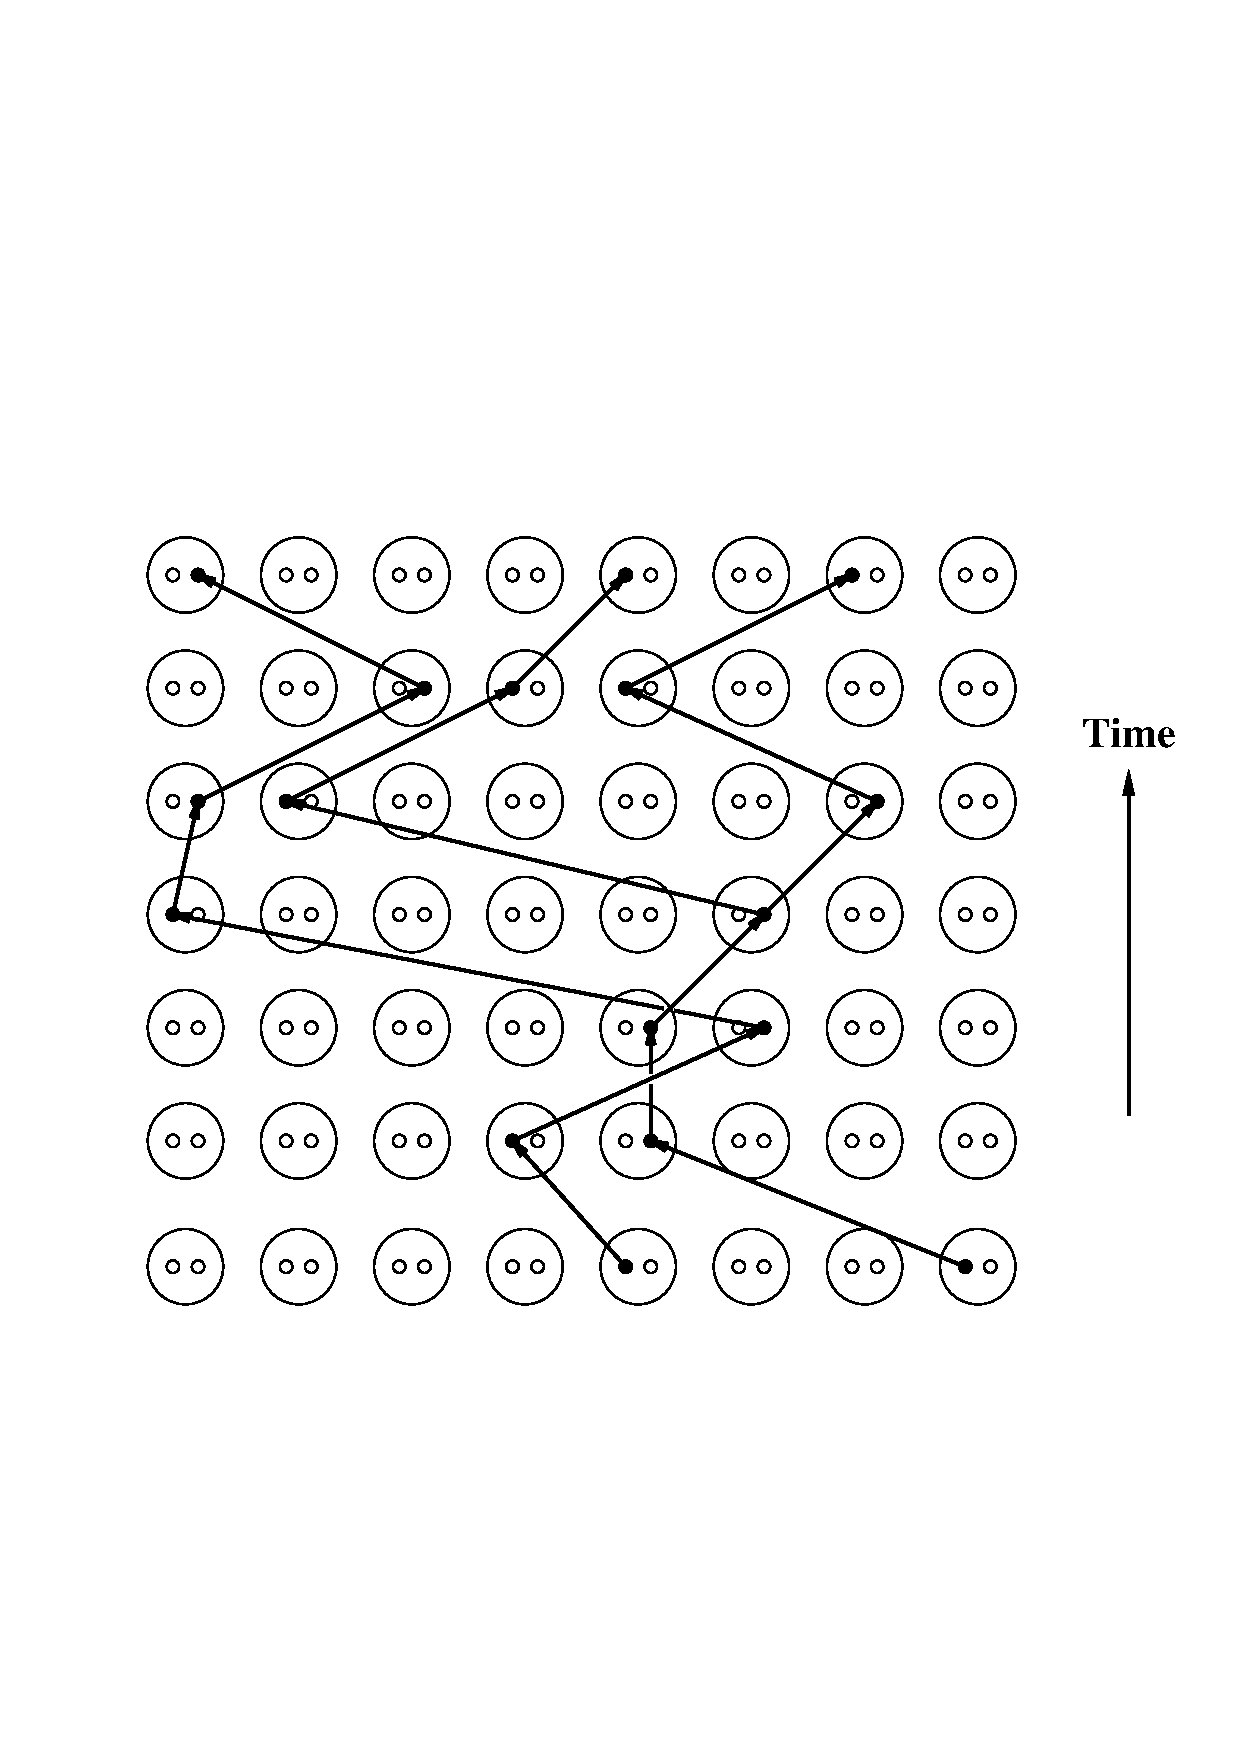
\includegraphics[width=6in]{fig1.pdf}}

\newpage

\centerline{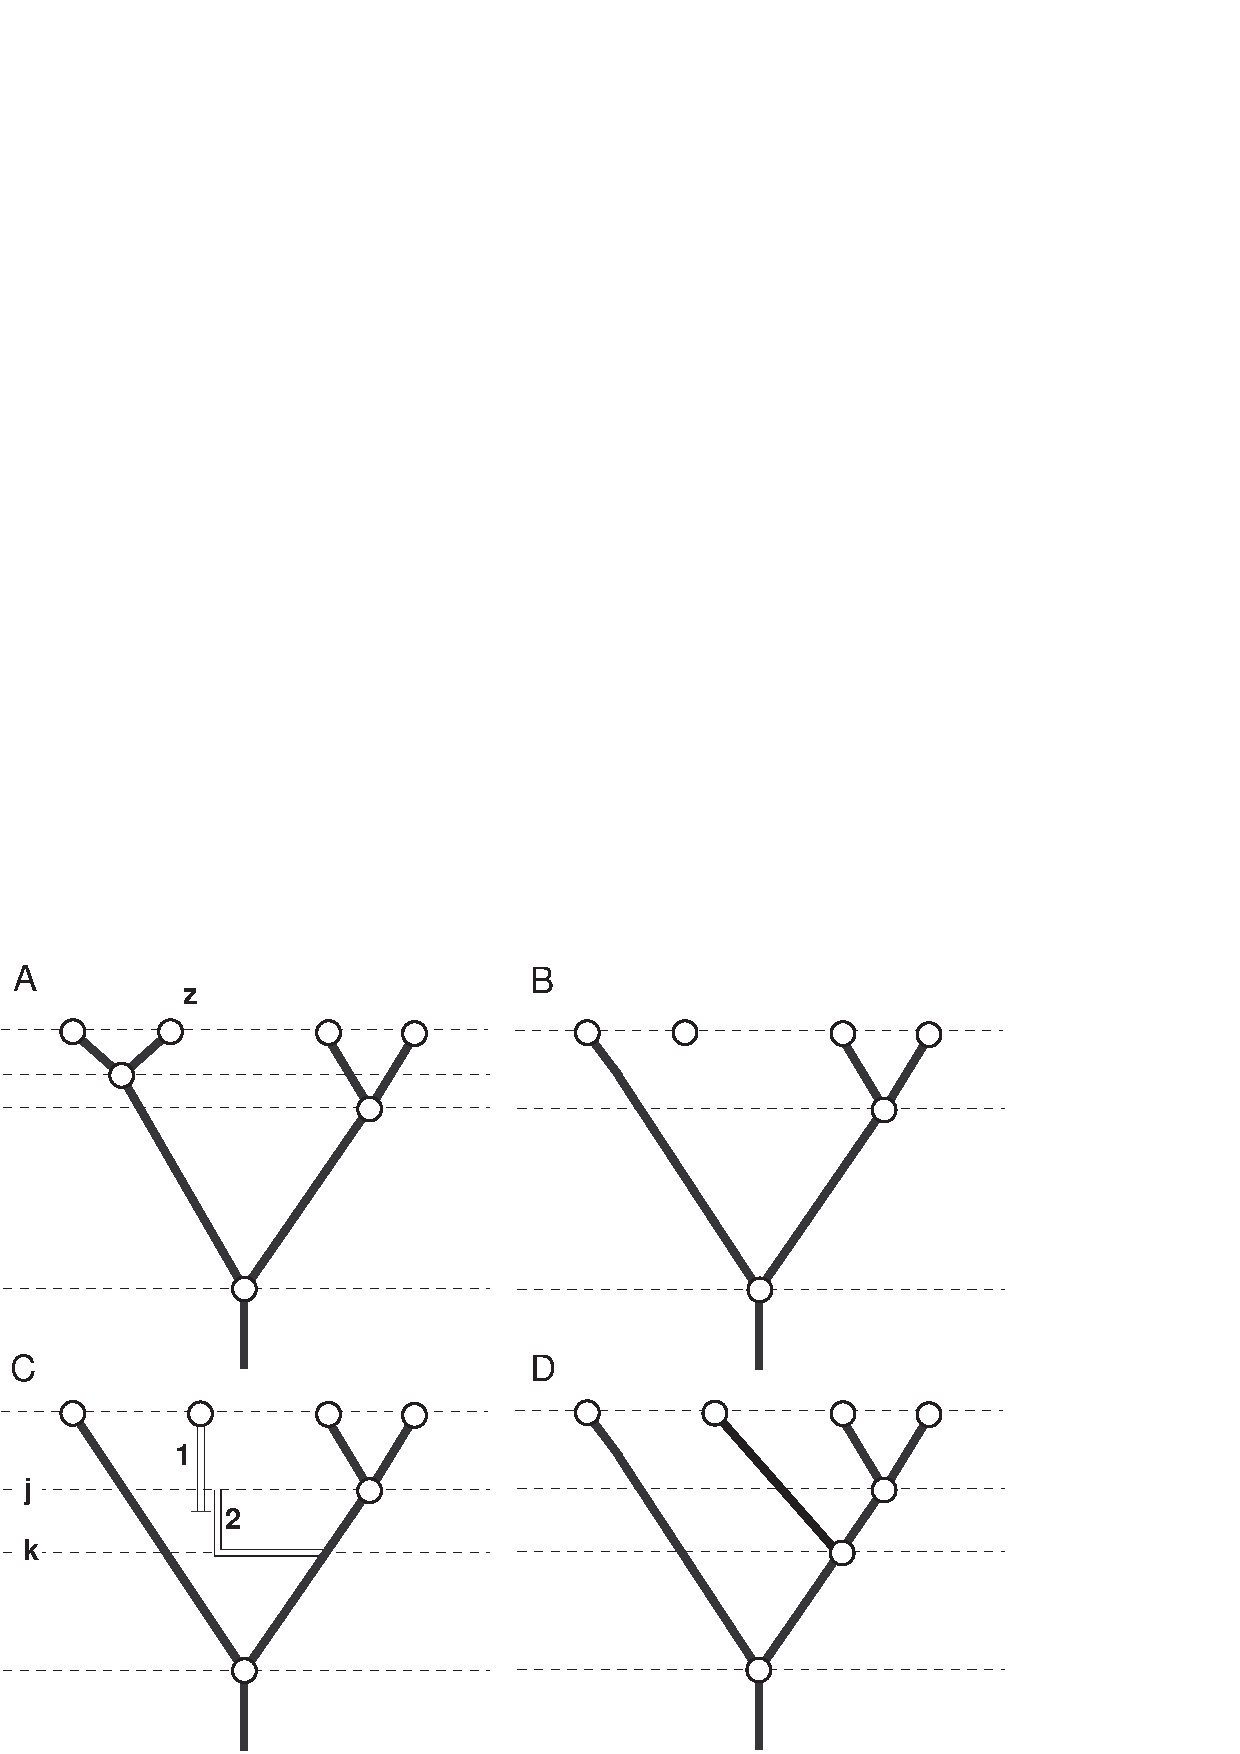
\includegraphics[width=5in]{fig2.pdf}}

\newpage

\centerline{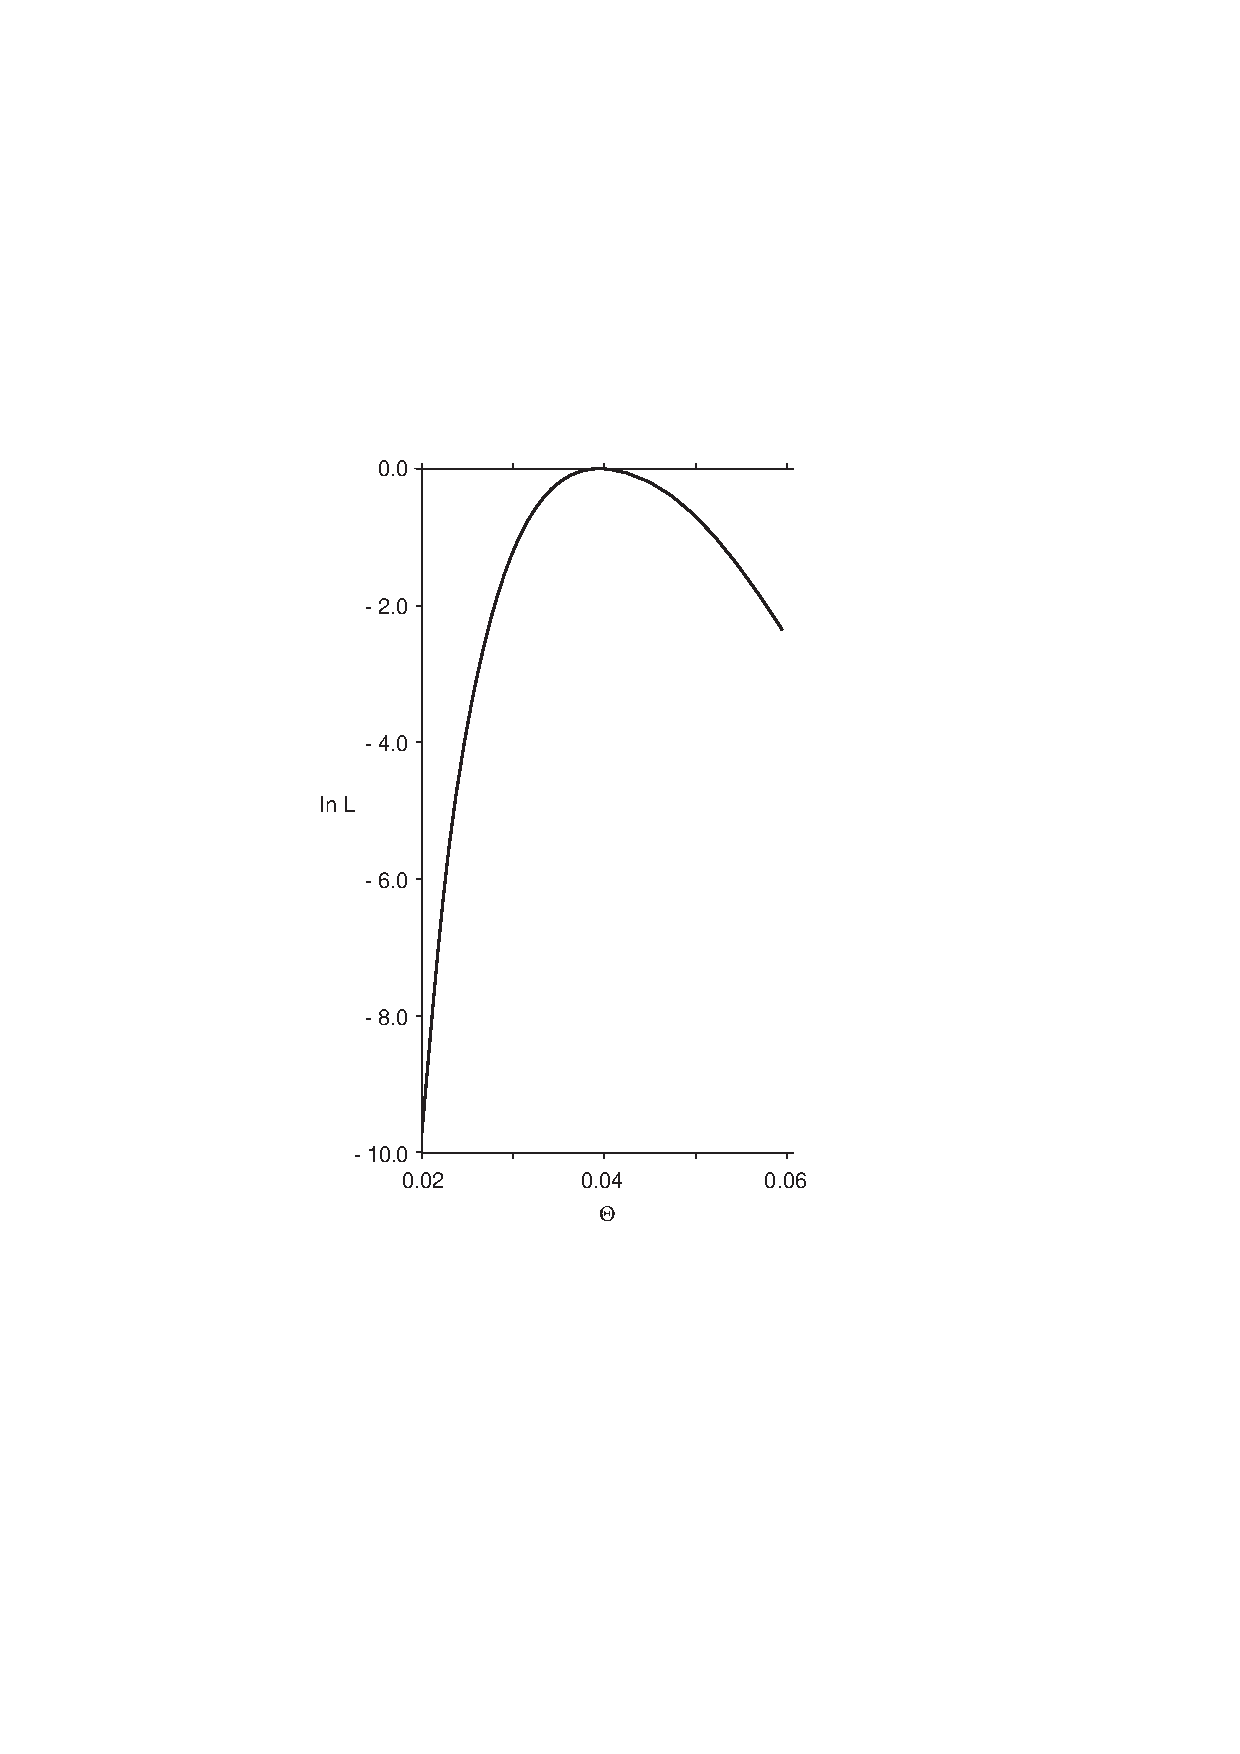
\includegraphics[width=7in]{fig3.pdf}}

\end{document}

